% !TEX root = main.tex
\chapter{Simulações e Resultados}
\label{cha:results}

Compreendendo e seguindo as etapas da publicação de Ian Goodfellow sobre GANs \citep{NIPS2014_5423}, uma versão primária do código foi escrita em linguagem Python sobre o Jupyter Notebook a partir do algoritmo publicado no artigo, e que também foi devidamente apresentada ao final do Capítulo \ref{cha:gan}.

Nenhum dos conjuntos de dados mencionados vem pronto para ser usado em um formato conveniente, por isso foi necessário prepará-los para serem utilizados. Com os conjuntos de dados já preparados, foi necessário definir as funções responsáveis pela escolha das amostras que deveriam ser utilizadas nos treinamentos e testes. Todas as implementações de aprendizado profundo que usaram tensores foram feitas usando \textbf{PyTorch} \citep{paszke2017pytorch} e \textbf{TensorFlow} \citep{abadi2016tensorflow}; ambas são bibliotecas, escritas em Python, preparadas para trabalhar com tensores e permitem que o processamento seja executado por Unidades de Processamento Central (CPUs) e Unidades de Processamento Gráfico (GPUs). É possível escolher se o processo deve priorizar que o processamento seja realizado por CPU ou GPU; este trabalho prioriza a execução por GPU.

As redes foram implementadas separadamente; uma classe para o Discriminador, $D$ e outra para o Gerador, $G$. Neste caso, ambas as classes usaram uma rede neural artificial de três camadas ocultas para suas operações. O método de otimização adotado é \textbf{Adam} \citep{kingma2014adam}, que é baseado em estimativas adaptativas de momentos de menor ordem. A etapa de treinamento foi estabelecida com 200 épocas e o conjunto de dados de treinamento foi dividido em 600 lotes de 100 amostras cada.

%   ----- DATASETS -----
\section{Datasets}
\label{sec:results_datasets}

Dois \textit{datasets} foram explorados para testar as implementações: \textbf{MNIST}\footnote{\textit{\textbf{M}odified \textbf{N}ational \textbf{I}nstitute of \textbf{S}tandards and \textbf{T}echnology} (\textbf{MNIST}).} \citep{lecun-mnisthandwrittendigit-2010} e \textbf{CIFAR}\footnote{\textit{\textbf{C}anadian \textbf{I}nstitute \textbf{F}or \textbf{A}dvanced \textbf{R}esearch} (\textbf{CIFAR}).} \citep{cifar-dataset}; ambos os \textit{datasets} serão melhor detalhados e explicados a seguir.

O MNIST é um conjunto de dados amplamente utilizado de números manuscritos com 70.000 exemplos (60.000 para o conjunto de treinamento e 10.000 para o conjunto de teste); é uma versão modificada de um subconjunto do conjunto de dados NIST original. Os números foram escritos por 250 escritores diferentes, e os escritores responsáveis pelo conjunto de treinamento não são os mesmos escritores que são responsáveis pelo conjunto de testes. Todas as imagens no MNIST foram normalizadas de uma caixa de 28x28 pixels (resolução) para uma caixa de 20x20 pixels, preservando sua proporção e, como resultado da técnica de anti-aliasing (do algoritmo de normalização), elas não são mais preto e branco , mas tons de cinza; o resultado teve seu centro de massa centrado novamente em uma caixa de 28x28 pixels.

Existem versões modificadas do MNIST que usam uma paleta de cores invertidas, tornando o número preto e o plano de fundo branco, mas a essência do conjunto de dados MNIST ainda seria preservada para os fins pretendidos. A figura \ref{fig:datasets_mnist} tem algumas amostras do dataset MNIST.

% MNIST
\begin{figure}[H]
    \centering
    \subfloat{
\includegraphics[width=0.175\textwidth]{figs/MNIST/mnist_0.pdf}}\hspace{0.1cm}
    \subfloat{
\includegraphics[width=0.175\textwidth]{figs/MNIST/mnist_1.pdf}}\hspace{0.1cm}
    \subfloat{
\includegraphics[width=0.175\textwidth]{figs/MNIST/mnist_2.pdf}}\hspace{0.1cm}
    \subfloat{
\includegraphics[width=0.175\textwidth]{figs/MNIST/mnist_3.pdf}}\hspace{0.1cm}
    \subfloat{
\includegraphics[width=0.175\textwidth]{figs/MNIST/mnist_4.pdf}}
    \\
    \subfloat{
\includegraphics[width=0.175\textwidth]{figs/MNIST/mnist_5.pdf}}\hspace{0.1cm}
    \subfloat{
\includegraphics[width=0.175\textwidth]{figs/MNIST/mnist_6.pdf}}\hspace{0.1cm}
    \subfloat{
\includegraphics[width=0.175\textwidth]{figs/MNIST/mnist_7.pdf}}\hspace{0.1cm}
    \subfloat{
\includegraphics[width=0.175\textwidth]{figs/MNIST/mnist_8.pdf}}\hspace{0.1cm}
    \subfloat{
\includegraphics[width=0.175\textwidth]{figs/MNIST/mnist_9.pdf}}    
    \caption{Amostras do \textit{dataset} MNIST.}
    \label{fig:datasets_mnist}
\end{figure}



%   ----- AMBIENTE DE SIMULAÇÃO -----
\section{Ambiente de Simulação}
\label{sec:results_simulation_environment}

A fim de melhorar as condições de reprodutibilidade das simulações realizadas neste trabalho, é importante observar a Tabela \ref{tab:results_pc_specs}, que traz as configurações do ambiente em que todas as simulações foram realizadas.

\begin{table}[H]
    \centering
    \caption{Ambiente de simulação.}
    \begin{tabular}{ll}
        \toprule
        \textbf{Componente} &   \textbf{Descrição}\\
        \midrule
        Processador         &   Intel Core i5-8600K 3.6 GHz (4.3 GHz Turbo) 6-Core 9 MB Cache\\
        \hline
        CPU Cooler          &   Corsair H80i v2 Water Cooler\\
        \hline
        Placa Mãe           &   Gigabyte Z370XP SLI\\
        \hline
        Memória RAM         &   Corsair Vengeance DDR4 3000 MHz 16 GB (2 
        x 8 GB) C15\\
        \hline
        SSD                 &   Kingston UV400 240 GB SATA III\\
        \hline
        SSHD                &   Seagate Híbrido Firecuda 2 TB 64 MB Cache 
        SATA III\\
        \hline
        Placa de Vídeo      &   EVGA GTX 1080 Ti SC2 11 GB\\
        \hline
        Fonte               &   Corsair CS750M\\
        \hline
        Sistema Operacional &   Ubuntu Desktop 18.04 LTS 64-bit\\
        \hline
        NVidia Driver       &   v418.43\\
        \hline
        CUDA                &   v10.1\\
        \hline
        CUDNN               &   v7.5\\
        \hline
        PyTorch             &   v1.0.1\\
        \bottomrule
    \end{tabular}
    \label{tab:results_pc_specs}
\end{table}

A respeito do processador, apesar de a frequência de operação de 4.3 GHz ser atingida apenas por meio da função Turbo, essa função pode ficar ativada sempre que o processador detectar uma demanda por alto poder de processamento, o que pode ocorrer durante todo o período de processamento da simulação. A refrigeração da CPU foi feita por meio de uma solução relativamente poderosa, assim como a fonte utilizada possui capacidades consideravelmente superiores às demandadas, além de ser altamente estável e suficientemente eficiente; isso garantiu que nenhum dos resultados tenha sofrido interferências negativas por conta de qualquer questão inesperada e atípica relacionada ao \textit{Hardware}. Apesar de o computador possuir um SSHD, que é uma solução híbrida, o sistema operacional, os programas utilizados e todos os arquivos dos \textit{datasets} localizavam-se no SSD; o SSHD foi apenas utilizado para fins de \textit{Backup}.

Embora o PyTorch ofereça suporte a processamento por GPUs, várias etapas que envolvem processamento somente podem ser efetuadas por CPU, o que, inevitavelmente, faz com que haja um aumento no tempo demandado para concluir toda a simulação. Essa constatação pode ser efetuada por meio de monitores de recursos do sistema operacional e da placa de vídeo; no caso do Ubuntu, eles podem ser acessados por meio dos comandos \textbf{\$ htop} e \textbf{\$ nvidia-smi}, sendo que, caso se deseje visualizar o monitor de recursos da gpu com um intervalo de atualização de 1 segundo, pode-se utilizar o comando \textbf{\$ watch -n 1 nvidia-smi}. Exemplos de ambas as ferramentas de monitoramento de recursos podem ser vistas na Figura \ref{fig:results_resources_monitoring_tools}.

\begin{figure}[H]
    \centering
    \subfloat[htop]
    {
        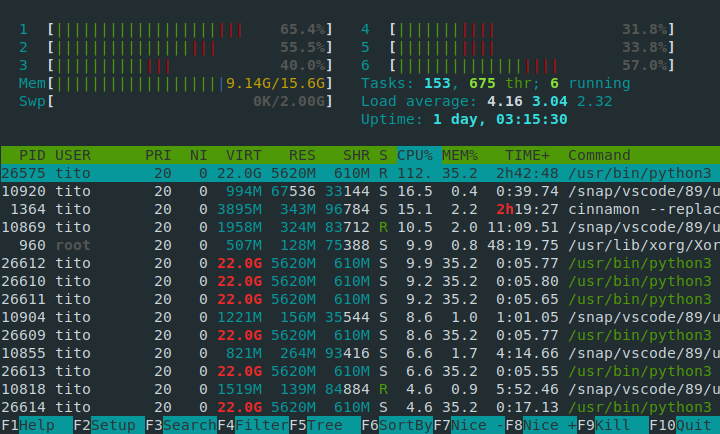
\includegraphics[width=0.75\textwidth]{figs/htop.png}
        \label{fig:results_htop}
    }
    \\
    \vspace{0.5cm}
    \subfloat[nvidia-smi]
    {
        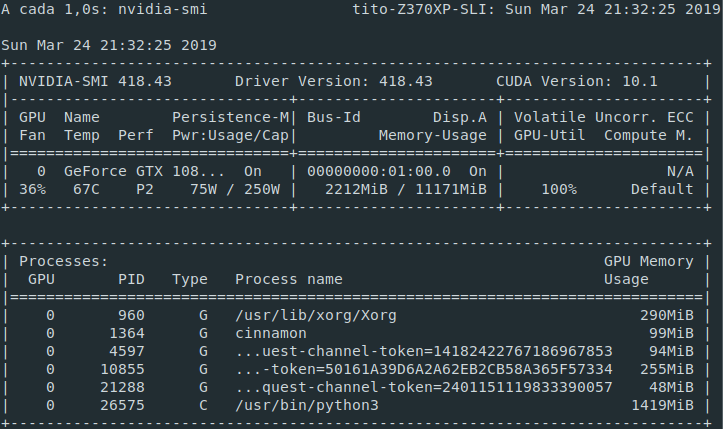
\includegraphics[width=0.75\textwidth]{figs/nvidia-smi.png}
        \label{fig:results_nvidia-smi}
    }
    \caption{Ferramentas de monitoramento, (a) htop e (b) nvidia-smi.}
    \label{fig:results_resources_monitoring_tools}
\end{figure}

A utilização de ferramentas de monitoramento de recursos se faz necessária para que seja possível averiguar a existência de qualquer eventual tarefa que, por qualquer razão que seja, esteja se utilizando dos recursos da máquina de modo a colocar em risco o desempenho da simulação. Diferentemente do que talvez se possa imaginar, atrapalhar a simulação não necessariamente significa apenas atrasar o término do processamento; em vez disso, pode significar eventuais alterações no comportamento do programa, o que poderia colocar em risco a veracidade dos resultados obtidos. Dito isso, é importante afirmar que nenhum comportamento maligno foi detectado ao longo das simulações.



%   ----- SIMULAÇÕES -----
\section{Simulações}
\label{sec:results_simulations}


\begin{figure}[H]
    \centering
    \subfloat[Época 0]
    {
        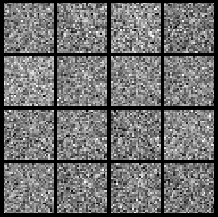
\includegraphics[width=0.30\textwidth]{figs/MNIST/new_tests/_epoch_0_batch_0.png}
        \label{fig:results_mnist_epoch-0}
    }
    \hspace{0.5cm}
    \subfloat[Época 3]
    {
        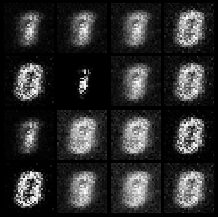
\includegraphics[width=0.30\textwidth]{figs/MNIST/new_tests/_epoch_3_batch_500.png}
        \label{fig:results_mnist_epoch-3}
    }
    \\
    \vspace{0.5cm}
    \subfloat[Época 32]
    {
        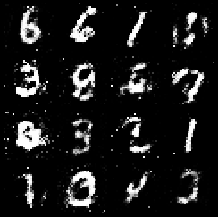
\includegraphics[width=0.30\textwidth]{figs/MNIST/new_tests/_epoch_32_batch_400.png}
        \label{fig:results_mnist_epoch-32}
    }
    \hspace{0.5cm}
    \subfloat[Época 299]
    {
        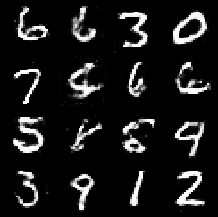
\includegraphics[width=0.30\textwidth]{figs/MNIST/new_tests/_epoch_299_batch_500.png}
        \label{fig:results_mnist_epoch-299}
    }
    \caption{Gerações da GAN \textit{Vanilla} para o \textit{dataset} MNIST em diferentes épocas.}
    \label{fig:results_mnist}
\end{figure}






\pagebreak
\newpage



\begin{figure}[H]
    \centering
    \subfloat[Erros]
    {
        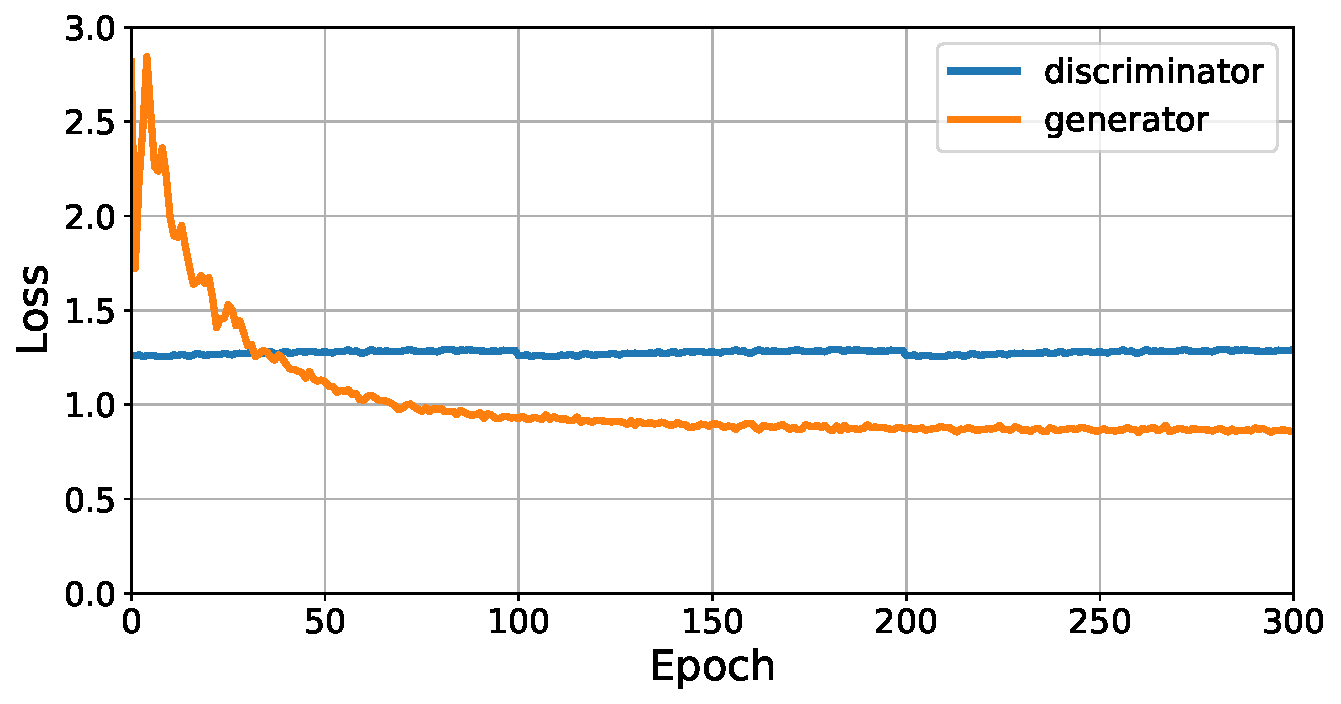
\includegraphics[width=0.75\textwidth]{figs/results/pytorch_vanilla_mnist_loss_0-299.pdf}
        \label{fig:results_pytorch_vanilla_mnist_loss}
    }
    \\
    \vspace{0.5cm}
    \subfloat[Incertezas]
    {
        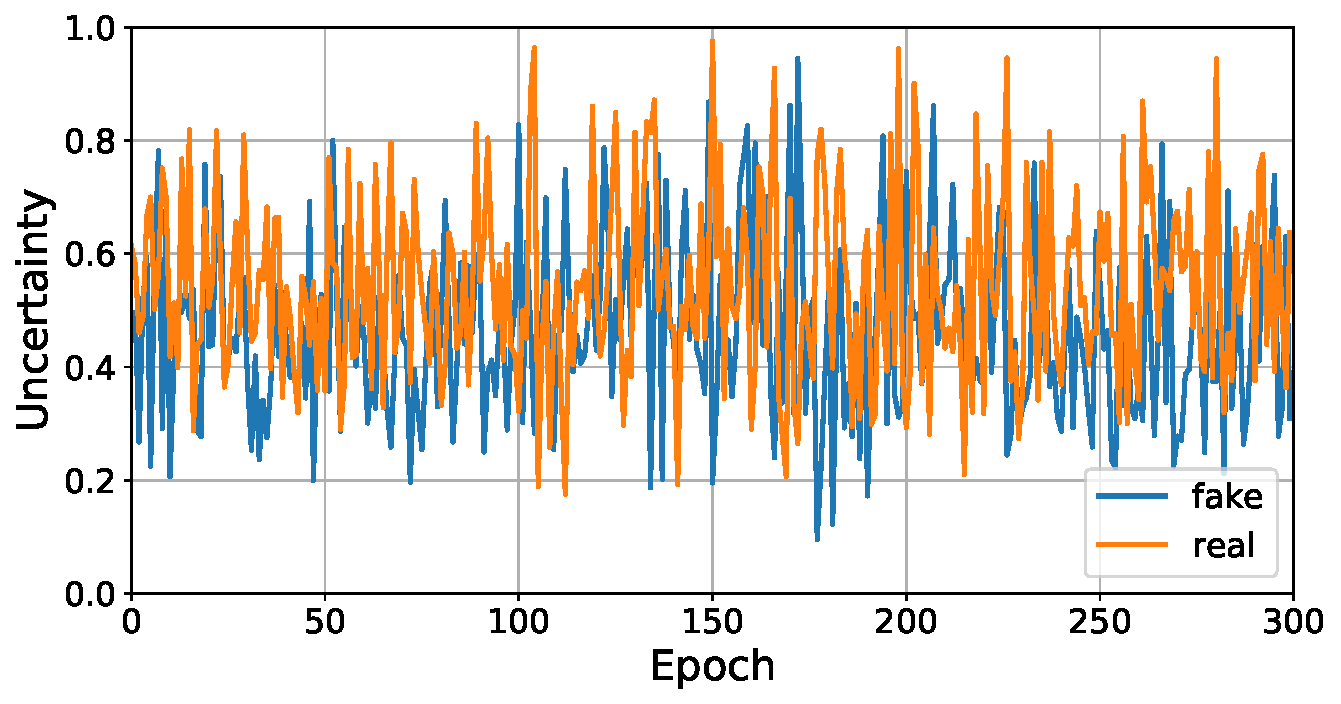
\includegraphics[width=0.75\textwidth]{figs/results/pytorch_vanilla_mnist_uncertainty_0-299.pdf}
        \label{fig:results_pytorch_vanilla_mnist_uncertainty}
    }
    \caption{Erros e incertezas da GAN \textit{Vanilla} para o \textit{dataset} MNIST em diferentes épocas.}
    \label{fig:results_pytorch_vanilla_mnist_scores}
\end{figure}